\section{Poisson pressure} % (fold)
\label{sec:poisson_pressure_driver}
The Poisson pressure provides a formulation to compute the pressure of a 3D domain related to its density structure. 
It is formulated as
$$
  \nabla \cdot \nabla p = \nabla \cdot (\rho \boldsymbol g)
$$
with $p$ the pressure (the unknown), $\rho$ the density and $\boldsymbol g$ the gravity acceleration vector.
This formulation presents the advantages of being fully 3D where lateral variations of density are well captured in the resulting pressure field, especially for non-hydrostatic cases.
More details can be found in (REF).
The discretisation is done on a $Q_1$ mesh overlapping the $Q_2$ mesh. 

\subsection{Boundary conditions} % (fold)
\label{sub:boundary_conditions}
The boundary conditions that can be used are
$$
  \hat{p}_1 \medspace \text{ on } \medspace \partial \Omega^M_1
$$
$$
  \nabla p \cdot \boldsymbol n = 0 \medspace \text{ on } \medspace \partial \Omega^M_2
$$
corresponding respectively to Dirichet and null flux.
In general, for geodynamics problem the approach is to set $\hat{p}_1 = 0$ along the top surface identified as \unix{JMAX\_LOC} in the \unix{DMDABCListTraverse3d()} method, and let the other boundaries to null flux; the natural Neumann condition in finite elements.
% subsection boundary_conditions (end)

\subsection{Driver options} % (fold)
\label{sub:driver_options}
The solve of this PDE can be done using its own driver \unix{\$\{PETSC\_ARCH\}/bin/test\_ptatin\_driver\_pressure\_poisson.app}.
This driver comes with its own options in addition to the standard other {\ptat} and {\PETSc} options.
Those are the following
\begin{itemize}
  \item \unix{-run}: runs the driver using the initial conditions described in the selected model
  \item \unix{-load}: loads a checkpointed job. The same rules than for checkpointing with the driver \unix{ptatin\_driver\_ts\_init.app} apply.
  \item \unix{-output\_vts}: directly outputs a \unix{.vts} file of the pressure field on the mesh in the path provided by the option \unix{-output\_path}. Without this option a petsc vec \unix{.pbvec} file is outputed and can be processed as all other raw files.
  \item \unix{-isostatic\_remesh}: Activates the use of a feature to compute the vertical displacement necessary to equilibrate the topography in agreement with the 3D density structure based on the poisson pressure field. This features comes with 2 \textbf{essential options}:
  \begin{itemize}
     \item[\textbullet] \unix{-isostatic\_density\_ref\_adim}
     \item[\textbullet] \unix{-isostatic\_compensation\_depth\_adim} 
   \end{itemize} 
  detailed in section \ref{sub:isostatic_remesh_functionnality}.
\end{itemize}
Additionally, the solver specific options can be set by prepending the prefix \unix{-LP\_} to standard {\PETSc} solver options.
% subsection driver_options (end)

\subsection{Isostatic remesh functionnality} % (fold)
\label{sub:isostatic_remesh_functionnality}
\begin{figure} [hbtp]
\center
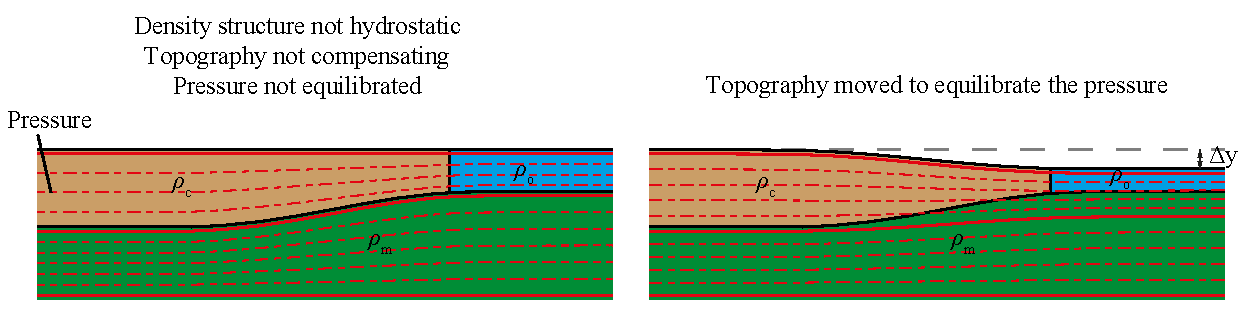
\includegraphics[width=0.8\textwidth]{figs/poisson_pressure.pdf}
\caption[\itshape ]
{\itshape Schematic representation (not to scale) of Left: an non-isostatically equilibrated topography and the pressure field associated with the density structure. Right: the same domain with a topography corresponding to an equilibrated pressure near the moho. The red lines are a representation of the pressure field. $\rho_c$, $\rho_o$ and $\rho_m$ stand for the density of the continental crust, the oceanic crust and the mantle.
}
\label{fig:pp_compensation}
\end{figure}
This functionnality introduces a general and simple way to approximate the topography generated by an non-hydrostatic density structure.
Such density structure are often related to ocean continent contacts and crustal thickness anomalies.
The approximation exploits a simple model based on the Airy isostatic model stating that at a given depth all pressures should be equilibrated. 
Therefore, while considering a constant pressure at surface (for instance $p=0$ at ground level), the density anomalies should generate topography to equilibrate the pressure in depth.
To get the displacement that should be generated to move the surface and accomodate the density structure, we compute 
$$
  u_y = -\frac{\Delta p}{\| \boldsymbol g\| \rho_{ref}},
$$
with $\| \boldsymbol g\|$ the norm of the gravity acceleration vector, $\rho_{ref}$ the density of the layer where the pressure should be equilibrated and $\Delta p = p - p_{ref}$ the difference between the pressure at the node located at the depth required by the user in the \unix{\{IMAX , JMAX\}} corner and the pressure at all other nodes located on the same $(x, z)$ plane of constant depth.
The resulting vector $\boldsymbol u = [0, u_y, 0]^T$ is stored as a {\PETSc} \unix{Vec} object in a \unix{.pbvec} file.

\subsubsection*{Options} % (fold)
\label{ssub:options}
To activate the fonctionnality add the option \unix{-isostatic\_remesh}.
In addition, come 2 mandatory options:
\begin{itemize}
  \item[\textbullet] \unix{-isostatic\_density\_ref\_adim}: the reference density ($\rho_{ref}$)  
  \item[\textbullet] \unix{-isostatic\_compensation\_depth\_adim}: the (minimum) depth at which the equilibrium should be reached. In order to have an effect on the topography, the chosen depth should not be too far from the deepest density variation. Otherwise, the pressure may not be perturbed enough to compute a significant topographic variation. 
\end{itemize}
Note that those 2 options require adimensionalised numbers (i.e., scaled by the scaling factor for density and length respectively).
To avoid passing adimensionalised arguments a possible way is to provide a custom user specific option, scale them user's model functions and add the scaled options at runtime with the {\PETSc} method \unix{PetscOptionsSetValue()}.
An example can be found in \unix{\$PTATIN\_DIR/src/models/poisson\_pressure\_model/model\_poisson\_pressure.c} in the function \unix{ModelSetIsostaticParameters()}.
% subsubsection options (end)

\subsubsection*{Required addition to user's model} % (fold)
\label{ssub:required_addition_to_user_s_model}
To be able to actually use the functionnality the users must add in their \unix{PTATIN\_MODEL\_APPLY\_INIT\_MAT\_GEOM} function pointer the call to \unix{LagrangianAdvectionFromIsostaticDisplacementVector(pTatinCtx ptatin)} performing the advection of the mesh surface and its remesh into an equally spaced grid and the advection of the material points. 
A special attention must be taken if a mesh refinement function is used, because the previous function overrides it during the advection.
In that case, provide the mesh refinement function right after the call of the advection function \unix{LagrangianAdvectionFromIsostaticDisplacementVector()}.
% subsubsection required_addition_to_user_s_model (end)

\subsubsection*{Procedure} % (fold)
\label{ssub:procedure}
To standard procedure to use this functionnality should be as follow:
\begin{lstlisting}
$PETSC_ARCH/bin/test_ptatin_driver_poisson_pressure.app -run -options_file path/to/options/file -isostatic_remesh -isostatic_density_ref_adim <density value> -isostatic_compensation_depth_adim <depth value> \
$PETSC_ARCH/bin/ptatin_driver_*.app -options_file path/to/options/file
\end{lstlisting}
The first job executes the poisson pressure driver, computes the vertical displacement and write it out in the \unix{output\_path} with the name (do not modify) \unix{isostatic\_displacement.pbvec}.
Then if the function \unix{LagrangianAdvectionFromIsostaticDisplacementVector()} is called in user's model (see sec \ref{ssub:required_addition_to_user_s_model}) the file is read during the model creation and applies the mesh and marker advection before any solve is performed.
% subsubsection procedure (end)
% subsection isostatic_remesh_functionnality (end)
% section poisson_pressure_driver (end)